% results_modelsize.tex
\subsection{Model Size and Structural Clarity}

A natural question is how much the embedding model's size matters. To show
the gradient directly, the same 50 items were embedded with three sizes of
the same model family---Qwen3-Embedding-0.6B (1,024 dimensions), 4B (2,560),
and 8B (4,096)---and the mean-centered Pearson similarity matrix was built
from each. Figure~\ref{fig:modelsize} shows the three matrices side by side,
items grouped by domain: the five diagonal blocks sharpen visibly with model
size, with the 0.6B matrix showing the haziest block boundaries and the 8B
matrix the crispest separation of within-domain from between-domain
similarity. Retention sharpens correspondingly. Under the 0.6B and 4B
embeddings the criteria disagree---parallel analysis retains \valPaKSmallWord{} and
\valPaKMediumWord{} factors, EGA \valEgaKSmallWord{} and \valEgaKMediumWord, for modal consensuses of
\valConsSmallWord{} and \valConsMediumWord---whereas under the 8B embeddings
parallel analysis and EGA converge on the theoretical \valPaKWord, and the
consensus is \valConsensusKWord{} (the eigenvalue-greater-than-one rule reports \valKaiserKWord{} and TEFI
\valTefiKWord{} at every size). Larger models of the same family thus yield semantic
structure that is both visibly cleaner and dimensionally closer to theory,
which is why the demonstration's main analyses use the 8B embeddings while
the package's on-device default remains the lighter 0.6B model.

\begin{figure}[H]
\centering
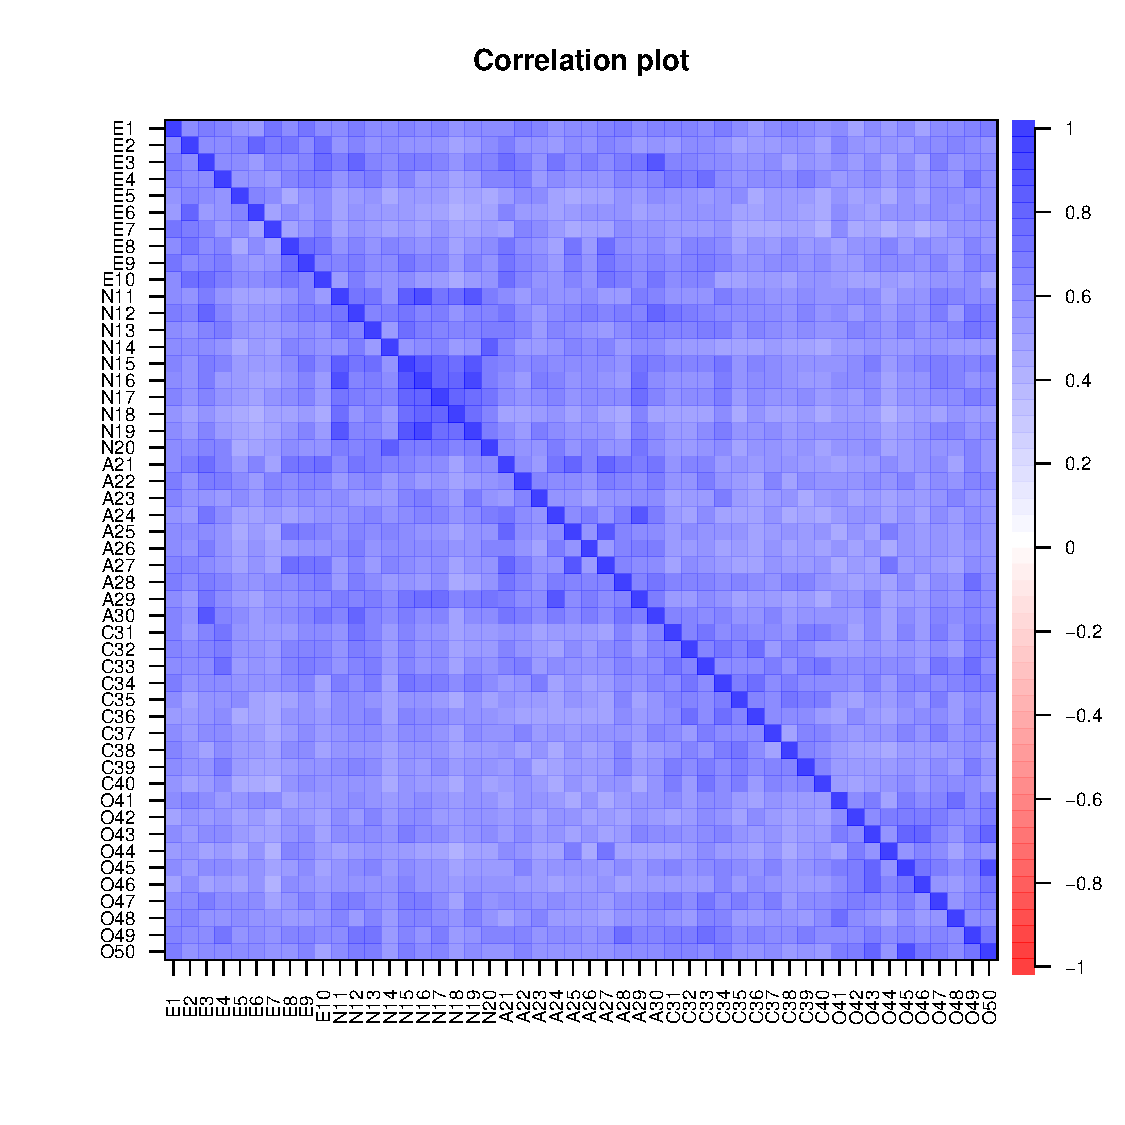
\includegraphics[width=0.32\textwidth]{figures/corplot_06b.pdf}\hfill
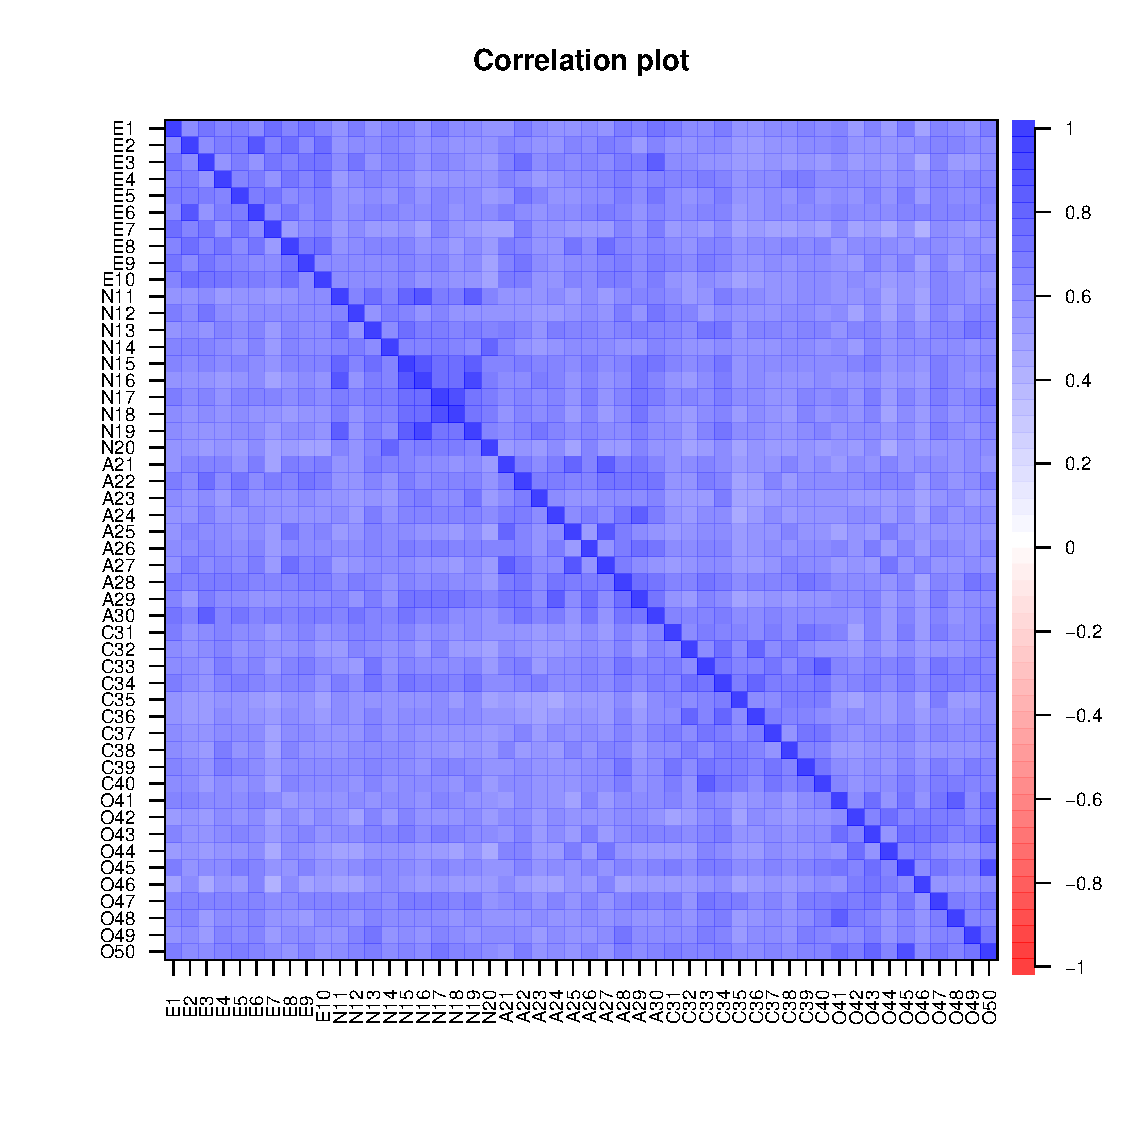
\includegraphics[width=0.32\textwidth]{figures/corplot_4b.pdf}\hfill
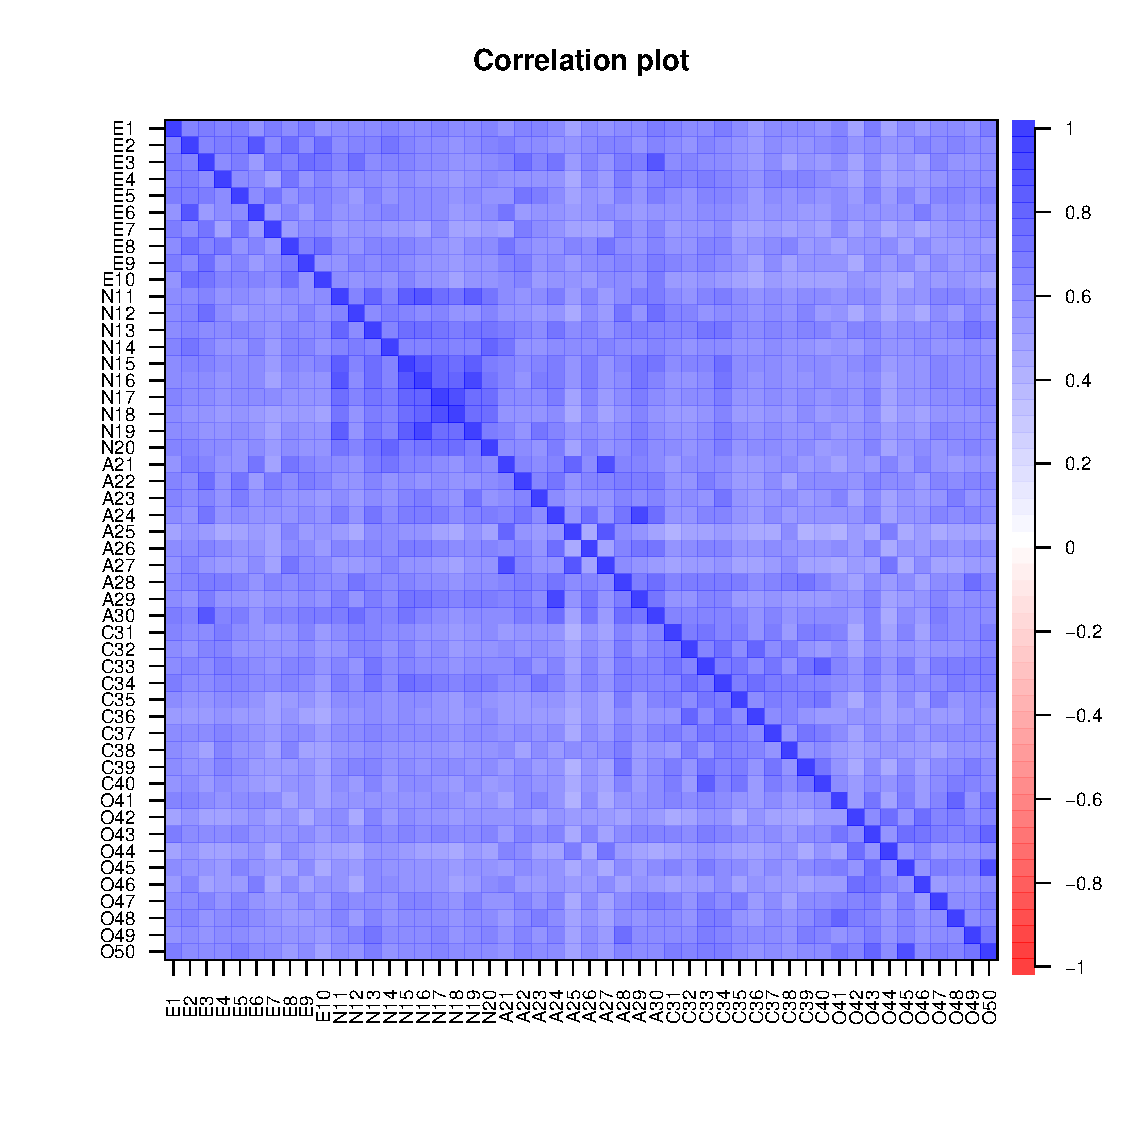
\includegraphics[width=0.32\textwidth]{figures/corplot_8b.pdf}
\captionsetup{justification=raggedright,singlelinecheck=false}
\caption{Mean-centered Pearson similarity matrices of the 50 IPIP items,
grouped by domain, for Qwen3-Embedding-0.6B (left), 4B (center), and 8B
(right). The domain block structure grows progressively crisper with model
size.}
\label{fig:modelsize}
\end{figure}
